\section{Literature Review}
\epigraph{\justify``We are drowning in data, but starving for knowledge.''}{John Naisbitt\\\textit{Megatrends, 1982}}

\subsection{Data-driven Astronomy}\label{sec:dda}
\begin{wrapfigure}{r}{0.2\textwidth}
	\centering
	\vspace{-\intextsep}
	\includegraphics[width=.2\textwidth, keepaspectratio]{images/misc/cannon.png}
	\caption{Annie J. Cannon at Radcliffe College \parencite{schlesinger_library_portrait_2016}}
	\vspace{-15pt}
\end{wrapfigure}
Humans are exceptional pattern matchers. Studies have shown that we are able to discern human faces within hundreds of milliseconds from first perceiving them \parencite{caharel_face_2013, barragan-jason_neural_2015}. Adapting this innate trait combined with the propensity to explain external reality, and with incisive reasoning; scientists have yielded groundbreaking discoveries. Consider the discovery of the laws of planetary motion by Johannes Kepler. The laws were the result of analysis of Tycho Brahe's comprehensive data on Mars' motion which he had catalogued diligently over two decades.

Likewise, Annie Jump Cannon (1863-1941) despite her hearing-impairment devised the stellar classification scheme also known as the `Harvard Spectral Classification' \parencite{wolbach_library_of_the_harvard-smithsonian_center_for_astrophysics_astronomy_2019}. With this scene, along with other human computers, she manually categorized a staggering quarter of a million stars.

As the efficiency of optics and computing technology catapults exponentially, the volume of data modern telescopes generates are dramatic. Within the last decade, surveys like the Sloan Digital Sky Survey and the Hubble Deep Field project have collected hundreds of terabytes of information \parencite[43]{ivezic_statistics_2014}. Criteria and heuristics are easily programmable while intuitions shown for example by Cannon is difficult to describe in a set of rules. As the rules grow with the complexity of the problem, it gets difficult to encapsulate the desired goal. Machine Learning addresses this issue by scaling learnability and applying the new-found knowledge to solve for unknown variables.

\subsection{Machine Learning - A Primer}\label{sec:mla}
\paragraph{Computational Pattern Recognition}
The term `Machine Learning' (ML) at its face value can seem oxymoronic to a layperson. How can insentient machines exhibit human attribute akin to learning? It cannot, in the way humans do. However, a more accurate definition would include the potential for computer programs to detect pattern or trend in a given sequence of data. Therefore, machine learning all in all can be mapped to algorithmic \emph{pattern recognition}.

\paragraph{Inductive inference}
Philosophers since antiquity have pondered upon and produced myriad frameworks for sound and valid inferences. From Aristotelian syllogism to the more extensive Fregean derivatives such as first-order predicate logic, the reasoning from induction has allowed to generalise out insightful functions from known data \parencite{thagard_philosophy_1990}. Tom Mitchell a luminary in Machine Learning from Stanford, states that the inductive learning hypothesis generates such generalisations and is one of the fundamental assumptions in ML to facilitate predictions \parencite*[23]{mitchell_machine_1997}. This philosophical abstraction is realized by two major steps in ML. 1) Read a dataset (measurements with correlations across various physical phenomena). And 2) Build a statistical model that describes the dataset. The model obtained is assumed (reasonably so) to work for new data.
\begin{figure}[H]
	\usetikzlibrary{positioning}
	\centering
	\tikzstyle{block} = [rectangle, draw, fill=blue!20, text centered, rounded corners, minimum height=2em]
	\tikzstyle{line} = [draw, -latex]
	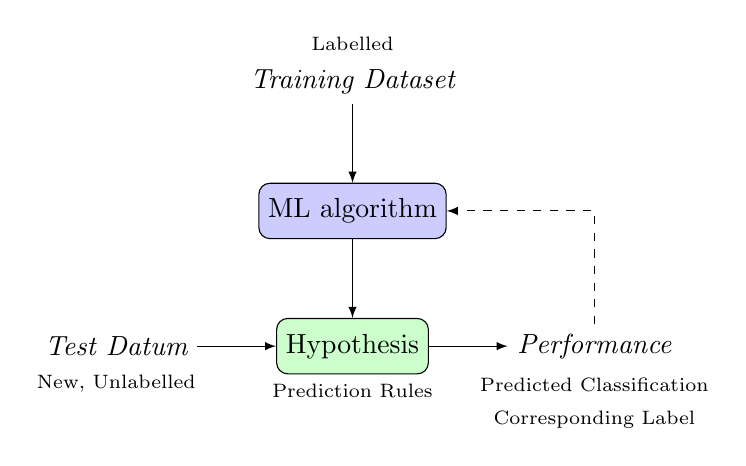
\begin{tikzpicture}
	\node[block] (ml) at (0,0) {ML algorithm};
	\node[label={90: \scriptsize{Labelled}}, above=of ml, font=\itshape] (trd) {Training Dataset};
	\node[label={-90: \scriptsize{Prediction Rules}}, block, fill=green!20, below=of ml] (h){Hypothesis};
	\node[label={-90: \scriptsize{New, Unlabelled}}, left=of h, font=\itshape] (td) {Test Datum};
	\node[label={[align=center]-90: \scriptsize{Predicted Classification}\\\scriptsize{Corresponding Label}}, right=of h, font=\itshape] (p) {Performance};
	
	\path[line] (td) -- (h);
	\path[line] (trd) -- (ml);
	\path[line] (ml) -- (h);
	\path[line] (h) -- (p);
	\path[line, dashed] (p) |- (ml);
	\end{tikzpicture}
	\caption{Machine Learning Process Abstraction}
	\label{fig:mlp}
\end{figure}
One of the earliest machine learning programs dates back to 1952 whence the AI pioneer, Carnegie Mellon professor Arthur L. Samuel (1901-1990) devised a remarkable computer game  in the IBM's Poughkeepsie Laboratory \parencite{stanford_university_professor_2019}. Samuel's checker's playing program could learn from past experience to improve its moves \parencite{mccarthy_memoriam:_1990}. His 1959 paper regarded seminal in the ML domain, set the groundwork for machine learning application and thus the term itself was coined for the first time \parencite{samuel_studies_1959}. Samuel's definition of machine learning can be recapitulated as the domain of computing that enables programs to learn without the input of active and explicit instructions. 

Modernizing Samuel's definition, the Carnegie Mellon computer scientist Tom Mitchell provides a more formal definition: `A computer program is said to learn from experience E with respect to some class of tasks T and performance measure P, if its performance at tasks in T, as measured by P, improves with experience E' \parencite*{mitchell_machine_1997}. Consider the example of a checkers playing machine learning program. This problem would be posed formally in Machine Learning terms as:

\begin{table}[h]
	\centering
	\begin{adjustbox}{width=\linewidth}
	\begin{tabular}{|l|l|l|}
		\hline
		Experience & \emph{E} & Experience of Checkers playing\\
		Task& \emph{T} & Playing Checkers\\
		Performance & \emph{P} & Probability of program's future victory\\
		\hline
	\end{tabular}
	\end{adjustbox}
	\caption{Mitchell's formalisation of checker's playing ML program\parencite*[6]{mitchell_machine_1997}
.}
\end{table}

\subsection{Machine Learning's Relation with other domains}
\begin{figure}[H]
	\centering
	\usetikzlibrary{,positioning}
	\tikzstyle{block} = [rectangle, draw, fill=blue!20, text centered, rounded corners, minimum height=2em]
	\tikzstyle{line} = [draw, -latex]
	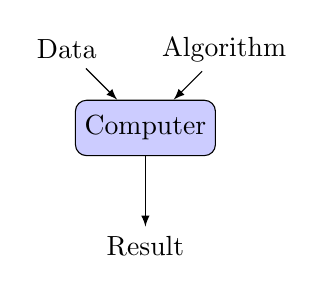
\begin{tikzpicture}
	\node (data) at (-1,0) {Data};
	\node(algorithm) at (1,0) {Algorithm};
	\node [block] (computer) at (0,-1) {Computer};
	\node (result) at (0,-2.5) {Result};
	
	\path[line] (data) -- (computer);
	\path[line] (algorithm) --(computer);
	\path[line] (computer) -- (result);
	\end{tikzpicture}
	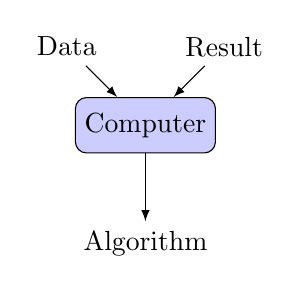
\begin{tikzpicture}[node distance = 2cm, auto]
	\node (data) at (-1,0) {Data};
	\node (result) at (1,0) {Result};
	\node [block] (computer) at (0,-1) {Computer};
	\node (algorithm) at (0,-2.5) {Algorithm};
	
	\path[line] (data) -- (computer);
	\path[line] (result) --(computer);
	\path[line] (computer) -- (algorithm);
	\end{tikzpicture}
	\caption{Traditional Programming vs Machine Learning}
	\label{fig:tml}
\end{figure}

At the onset, it is crucial to differentiate traditional computing with machine learning. As depicted in the figure above, the results and raw materials generating them are conspicuously the inverted reflections of each other. However, programming is not replaced by machine learning. Rather they exist concurrently, and work complementing each other. The former solves the computational problem where the rules are known before-hand, and the later solves problems based on experience as heuristics programming is not possible for certain problems \parencite{mitchell_machine_1997}.

Another important distinction is of that between AI and Machine Learning. The term Artificial Intelligence (AI) and Machine Learning are sometimes used interchangeably in a colloquial setting. Pedro Domingoes, professor of computer science and engineering at the University of Washington illuminates the relationship between big data, artificial intelligence, and machine learning in the analogy as follows. Take for example a planet that we want to inhabit for noble reasons. The space shuttle that we build to reach the planet can be taken as machine learning. The fuel in the fuel tank attached to the shuttle is the big data. And the destination is artificial intelligence \parencite*{domingos_what_2019}. Hence, machine learning is a means to achieve artificial intelligence. And the fuel that drives machine learning is big data.

During the last six decades for which AI has been around, it went through cycles of ebb and flow. From the 1980s to 1990s, AI suffered from the last bust cycle. Much of the theoretical underpinnings were difficult to materialise and the research fundings waned as the delivery and hype were discordant. These bust periods were known as the `AI Winters' \parencite{rebala_introduction_2019}. Such winters were later overcome by the advent of machine learning and its success in solving real-world problems in classification, regression, and clustering.

With regards to machine learning's relation to data mining, Tom Mitchell provides a helpful description. He subsumes machine learning into the data mining process which has the goal of knowledge discovery from large datasets. Machine Learning is one of the important tools in data mining used to train a model that represents the dataset. Other tools and processes include database management, data cleansing, data visualisation, and empirical regularity analysis. This data mining acts as a bridge to connect many technical areas including statistical analysis, machine learning, and informatics\parencite*{mitchell_machine_1999}.

\subsection{Types of Machine Learning Problem}
Not all problems are machine learning solvable. The problems that can be addressed by the Machine Learning algorithm is broadly categorised into three categories. This is illustrated below, along with their subcategories. in figure \ref{fig:mlt}

\begin{figure}[H]
	\centering\
	\begin{adjustbox}{width=\linewidth}		
	\begin{forest}
		for tree={
			rounded corners, draw, align=center, top color=white, bottom color=blue!20,
			edge+=->,
			l sep'+=8pt,
		}, 
		[Machine Learning Problem,bottom color=green!20[Supervised[Regression, bottom color=gray!20][Classification, bottom color=gray!20]][Unsupervised[Clustering, bottom color=brown!20]][Reinforcement]]
	\end{forest}
	\end{adjustbox}
	\caption{Types of Machine Learning Problem}
	\label{fig:mlt}
\end{figure}

\subsubsection{Supervised Learning}
\begin{figure}[H]
	\centering
	\frame{\includegraphics[width=.7\linewidth, keepaspectratio]{images/misc/SL.png}}
	\caption{Supervised Learning: (1) Feature Extraction (Labelled Data) (2) Learning (Model learnt using for example the decision tree ID3 algorithm) (3) Prediction}
\end{figure}
In \textbf{supervised learning}, the machine learning algorithm is input the \textbf{dataset} of \textbf{labelled examples} where the mapping between parameter features and target features are realized. The collection of labelled examples can be stated as: ${(x_i, y_i)}^N_{i=1}$, where $x$ is the input feature, $y$ is the target corresponding target feature, the subscript $i$ is the index, and $N$ is the dataset size \parencites[21]{mitchell_machine_1997}[263]{guttag_introduction_2016}.

Each element $x_i$ in the $N$ space is also known as the \textbf{feature vector}. Feature vector in which its dimension can range from $j=1,\ldots,D$ is reasonably assumed to describe the given example. The value it holds is called a \textbf{feature} and is denoted as $x^{(j)}$. Consider, for example, a collection of students' data. If each example $x$ in the collection represents a student, then his or her features could be stored as first feature $x_{(1)}$ could be the course enrolled in as string, the second feature $x_{(2)}$ could contain the gender as character M for male and F for female, the third $x_{(3)}$ could contain the academic year enrolled and so on. The feature vector always contains homogeneous information on feature at the position $j$ for every example in the dataset. This is to say that, if $x^{(3)}_2$ contains the information on gender, M or F in certain example $x_i$, then $x^{2}_k$ will also contain the gender information in every example $x_k$ where $k=1,\ldots,N$.

The label $y_i$ is the \textbf{target vector} or the information that is predicted about an example. It can be an element belonging to a finite set of classes ${1,\ldots, P}$ or// $\{`Malignant', `Benign'\}$ for breast tumour case, or a real number, or a complex object like a vector, tree, or a graph. A \textbf{class} is a category to which the example belongs to. For instance, if the examples are the galaxy types based on its shape then the classes can be $\{elliptical, spiral, lenticular\}$

Supervised learning algorithm has one goal which is to learn from a dataset and produce a \textbf{model} that takes feature vector $x$ and outputs information $y_i$ that corresponds to the feature vector. For instance, a model created using the diagnosed patient's dataset can input feature vector representing the patient such as age, tumour size, and tumour hardness and the output can be the probability of whether the person has a benign or a malignant tumour.

\subsubsection{Unsupervised Learning}
\begin{figure}[H]
	\centering
	\frame{\includegraphics[width=.7\linewidth, keepaspectratio]{images/misc/UL.png}}
	\caption{Unsupervised Learning: (1) Feature Extraction (Unlabelled Data) (2) Learning (Model learnt using for example the Clustering Algorithm) (3) Prediction (Model applied to new data.)}
\end{figure}
Unsupervised learning is applied to \textbf{unlabelled examples} denoted as: $\{x_i\}^N_1$. Here again, x is a feature vector. The goal of unsupervised learning algorithm is to create a model that takes in a feature vector X and outputs a transformation of input another vector or into a value that can be further used for a practical purpose \parencite[264]{mitchell_machine_1997}; \parencite[264]{guttag_introduction_2016}. 

The goal of the unsupervised learning algorithm is to discover some latent structure in the input set of feature vectors. For instance, given a set of animal feature vectors, the unsupervised learning algorithm may separate the animals into nocturnal or diurnal, perhaps into amphibians or mammals. One of the widely used supervised learning techniques is known as clustering where similar feature vectors are clustered together and partitioned. Geneticists, for instance, can employ clustering to discover groups or patterns of similar genes \parencite[265]{guttag_introduction_2016}.

\newpage
\subsubsection{Reinforcement Learning}
\begin{wrapfigure}{r}{0.4\linewidth}
	\centering
	\tikzstyle{block} = [rectangle, draw, fill=blue!20, text centered, rounded corners, align=center, minimum height = 2em]
	\tikzstyle{block2} = [rectangle, draw, fill=green!20, text centered, rounded corners, align=center, minimum height=2em]
	\tikzstyle{olap} = [fill=white, text centered, align=center]
	\tikzstyle{line} = [draw, -latex]
	\usetikzlibrary{positioning}
	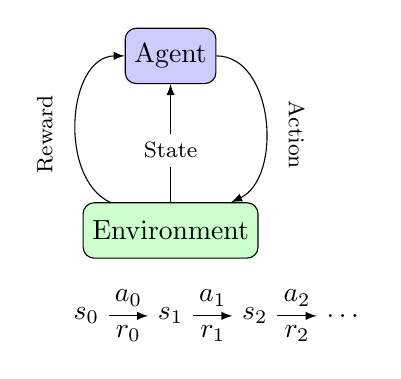
\begin{tikzpicture}[node distance=1.5]
	\node[block] (agent) {Agent};
	\node[block2, below = of agent] (env){Environment};
	\path(env)edge[line, out=155,in=180](agent.west) node[rotate=90] at (-1.6,-1){\footnotesize{Reward}};
	\path[line](env)--(agent)node[olap] at (-0,-1.2){\footnotesize{State}};
	\path(agent.east)edge[line, out=0,in=25](env) node[rotate=-90] at (1.6,-1){\footnotesize{Action}};
	
	\node[below = .5cm of env](s1){$s_1$};
	\node[left= .5cm of s1] (s0) {$s_0$};
	\node[right = .5cm of s1](s2){$s_2$};
	\node[right = .5cm of s2](s3){\ldots};
	
	\path[line](s0)--node[above]{$a_0$} node[below]{$r_0$}(s1) ;
	\path[line](s1)--node[above]{$a_1$} node[below]{$r_1$}(s2);
	\path[line](s2)--node[above]{$a_2$} node[below]{$r_2$}(s3);
	\end{tikzpicture}
	\caption{State Machine Representation of an Agent Interacting with its Environment.}
	\vspace{-10pt}
	\label{fig:rei}
\end{wrapfigure}
Reinforcement learning employs the most unique strategy in all learning classes. The machine or \textbf{agent} is said to live in its \textbf{environment} and able to interact with it and change its \textbf{state} as a vector of features. The interaction is done in a series of \textbf{actions}. Different actions elicit different \textbf{rewards} for the agent and in the process could change its state. The goal of reinforcement learning is to discover a \textbf{policy}. A policy, similar to the model in supervised learning is a function that takes in feature vector of states and outputs an optimal i.e. maximized average reward inducing action to execute.

In figure, \ref{fig:rei} an agent lives in an environment. At an instance, it exists in a particular state $s_i$ from a class of possible states $S$ and performs an action $a_i$ from a set of actions $A$. The agent gains real-valued reward $r_i$ for each action executed. The overall parameters produced are a sequence of states $s_i$ the associated each action $a_i$, and the instantaneous rewards for the action represented as $r_i$. The agent's goal is to learn an optimum control policy, $\Omega:S\rightarrow A$, that maximizes the average rewards in the sequence \parencite[367-370]{mitchell_machine_1997}.

\subsection{Ensemble Method}
Our social learning behaviour is characterised by accumulating expert advice from multiple sources before making a crucial decision. The combination of myriad \textbf{`experts'} to attain  \textbf{`ensemble'} decision has its roots in ancient Greece. The \emph{Conduret Jury Theorem}, which formalises this notion during the enlightenment age, proved that the collective judgement of expert individuals are superior compared to the individual expert opinion \parencite{de_condorcet_essai_2014}. Certain techniques known as the ensemble method attempts to mimic this social learning behaviour to attain a more reliable prediction.

In machine learning, ensembles are a finite set of learning machines that combines the different learning algorithms and perspectives on a dataset to obtain more reliable and accurate predictions in supervised and unsupervised learning, in contrast to a single learning machine's performance \parencite{dietterich_experimental_2000}; \parencite{kuncheva_combining_2014}. An example among many techniques on how this is achieved is the \emph{majority vote} ensemble method, which employs several different learning algorithms on a dataset and maintains a record of count on each classification label for which the individual algorithm proposed true result \parencite{cooper_when_1993}. The maximum count is then selected to the final true class for the prediction.

\paragraph{Literature Interests}
The literature of astronomical machine learning is rife with the alternative terms of ensemble \parencites{drucker_boosting_1994, filippi_multi-layer_1994, sung-bae_cho_multiple_1995, lam_optimal_1995, kittler_combining_1998, bunke_multiple_2002, banfield_comparison_2007}. Terms used interchangeably with the ensemble (widely recognized term in AI) include committee, fusion, aggregation, and combination. They all mean the same process of machine learning where multiple machines work together as opposed to the individual machine. In this dissertation, I have consistently used the word ensemble to mean this concept.

One of the major areas of interest within machine learning is in the field of ensemble methods \parencites{dietterich_experimental_2000, kuncheva_combining_2014} This is evinced in the workshops, paper presentations, and conferences devoted to this single topic. One prominent conference is spearheaded by Kittler et al. called the Multiple Classifier Systems (MCS) \parencites{guyer_cambridge_1992, benediktsson_multiple_2009, roli_multiple_2004, oza_multiple_2005, haindl_multiple_2007}. The efficacy of ensemble methods has been empirically studied and the experimental data against benchmark results show that they are significantly reliable than a single classifier \parencites{banfield_comparison_2007, dietterich_experimental_2000, sohn_experimental_2007}. There seem to be two major drivers for motivation for research into ensemble methods. First is, given the verified efficacy the status quo of affordable and fast computing, and powerful networks of workstations. And second is the deeper intellectual reasons to explore intrinsic characteristics of ensemble method \parencite[564]{way_advances_2012}.

There are also several theories proposed explaining the successful employment of ensembles. For instance, Breiman and Friedman's bias-variance analysis using the stochastic determination theory \parencite{breiman_bias_1996}, Kleinberg's stochastic determination theory \parencite{kleinberg_algorithmic_2000}, and the interpretation ensemble's improved generalisations by Allwein, Schapire, and Singer in light of the large margin classifiers \parencite{allwein_reducing_2001}.

Ensemble method employed in Astronomy is explicated in section \ref{sec:ema}

\subsection{The Origin of the Universe}
One of the earliest determiners for the expanding universe is the result of Edwin Hubble's meticulous observations of galaxies. Redshift encapsulates the phenomena of galaxies apparently moving away and is one of the myriad significant phenomena along with cosmic microwave background radiation, that proved the phenomenon of expanding universe. In 1929, Hubble proved that distant galaxies exhibited Doppler effect as their optical spectra showed a redshift in the emitted light \parencite*{hubble_relation_1929}. This was a clear indication that galaxies were moving away from the point of sight and in-fact every cosmic object was flying apart as the space between them stretched. If one were to rewind the cosmic movie of expanding universe, then there would come a point when everything would collapse back at a singular point known as the singularity which is the boundary of space, time, matter, and energy \parencites[18]{craig_ultimate_1999, davies_god_2007}.

\subsection{Redshift Measurements}
One of the frustrations of an observational science like astronomy is we can't set up experiments in the lab. It is not possible to control the unknown parameters to test hypotheses or use physical equipment like rulers to measure distances. Instead, a cleverly constructed observations are required to collect data that will help answer such questions. A redshift defectively gives us a distance to a galaxy and so by doing this, we can map out the universe in 3D\parencite{filippenko_great_2007}. Measuring spectroscopic redshift is the most accurate way of doing this but there are more galaxies for which imaging observations over spectroscopic ones are available. So a set of galaxies with known redshifts used for training the machine learning classifier to calculate redshifts for new sets of galaxies. This is the type of problem that machine learning is perfect for \parencite{ivezic_statistics_2014, way_advances_2012}. This is the task where astronomical elements are well understood, but it is not possible to do it with a rule-based approach.

Machine learning is a fast solution that allows us to evaluate the accuracy of the results and work out the probability of the results being correct. It can often seem like there's lots of hidden voodoo going on in machine learning. But really all we're doing is building a model based on known data and then applying that model to unknown data. In this study, I am able to calculate redshifts for the hundreds of thousands of galaxies. effectively using them as a tool to measure distance in the universe. But before the actual mechanics, theoretical foundations and the literature needs to be layed out.
 
 It is quite straightforward to calculate the redshift of the galaxy. In the presence of spectral fingerprint of elements in the earth that are also found in galaxies, the redshift is obtained by subtracting the elemental spectrograph data into the observed galaxy's spectrograph data. an example is shown in figure \ref{fig:rsp}. However, the process can be time-consuming and tedious for large samples. Likewise, without the reference and when the only spectrum for the galaxy is available it can be difficult to estimate the photometric shifts. This is where machine learning can help. Given the accurately calculated spectrum for other galaxies, the ML model is able to predict the redshifts in new galaxies.

Five decades ago Baum proposed the first measurement scheme for spectral energy distribution involving six elliptical galaxies. Uncharted territories were traversed for the first time when he later used photometry instead of spectroscopy to measure the redshifts \parencite[325]{way_advances_2012}.

\subsection{Galaxy Classification}
The \nth{18}-century philosopher Emmanuel Kant marvelled at what he called `the moral law within and the starry heavens above' \parencite[1]{kant_kant:_2012}. The former aspect in the dictum is encapsulated in his noted discourses in epistemology, ethics, and metaphysics.

\paragraph{The Nebulae Debate}
While the later which is lesser-known aspect is evinced in his theoretical studies in Astronomy. During the 1920s, a debate raged between astronomers about the massive fuzzy accretion in the night sky called the `nebulae'. Some believed they were clouds of local stars within the milky way, while others contested that they were extragalactic star systems. The latter camp was proposed centuries before the debate and before the existence of telescopes, by Hubble \parencite{hubble_realm_2013}.

\paragraph{Classical Classification}
Putting the nebulae debate to perpetual rest, Hubble had devised the first classification scheme for galaxies based on their morphology \parencite*{hubble_relation_1929}. It was based on the conspicuous physical feature of the galaxies observed. The ones with the bulge were labelled `Early-Type Galaxies (ETG)', whereas the others with the prominent disc were labelled `Late-Type Galaxies (LTG)'. His classification scheme is shown below in figure \ref{hdv}.
\begin{figure}[H]
	\centering
	\includegraphics[width=\linewidth, height=\textheight, keepaspectratio]{images/galaxies/ddiagram.png}
	\caption{Hubble-De Vaucouleurs Morphological Classification Scheme of Galaxies}
	\label{hdv}
\end{figure}
The spiral galaxies are further forked into barred (SB) and non-barred (S). De Vaucouleurs further refined the classification by adding T-Type numbers to further divide the spirals and ellipticals based on their spirality and ellipticity strengths respectively. All modern forms of galaxy classification schemes are the extended forms of the Hubble Sequence.

\paragraph{Evolution Misconception}
One of the popular misconceptions about the Hubble Sequence is that it depicts an evolutionary sequence of galaxies from the ellipticals on the left evolving to morph into one with a disk. However, Hubble, himself in his seminal work advised that `temporal connotation is made at one's peril' and further he explains his scheme is without prejudice of the evolution of galaxies \parencite[277]{hubble_realm_2013}.

Since Hubble's classification scheme, there have been numerous take on updating it \parencite{buta_galaxy_2013}. But, the core of the scheme remains intact with only minor changes. What has significantly changed is the acceleration in the number of galaxies classified using the scheme and still a massive number of galaxies yet to be classified. Following at the footsteps of Hubble, and with the transition of astronomers from visual photographic plate inspection to modern powerful telescopes and detectors, detailed morphologies have been produced and the results published. Significant catalogues include, The Hubble Atlas of Galaxies \parencite{sandage_hubble_1984}and the Third Reference Catalogue of Bright Galaxies (RC3) \parencite{vaucouleurs_third_1991}. These and other catalogues are available at and maintained by the NASA/IPAC Extragalactic Database \parencite{jet_propulsion_laboratory_california_institute_of_technology_home_2019}.

\paragraph{Imperative for Machine Learning Approach}
The problem with expert classification is the implausibility and infeasibility of classification due to the sheer size of the galaxy dataset. Consider for example the galaxy data collected by the Sloan Digital Sky Survey (SDSS). It exceeds in the figures of millions and cannot be visually inspected even by the ensemble of expert astronomers at work concurrently \parencites{strauss_spectroscopic_2002,york_sloan_2000}. It was conspicuous that an automated classifier system was required to solve this issue. However, traditional computer programming would not be able to take account the complexities of galaxies' shapes such as the differences in attributes such as spiralities, bars, bulges, brightness and disks \parencite[216]{way_advances_2012}.

\paragraph{Automated Classification Proposals}
One of the earliest automated galaxy classification scheme according to their morphology can be traced back to the proceedings of the astronomy conference entitled: `Le Monde des Galaxies' (The World Of Galaxies) which was held in 1989, April 12 -14 in the Institut d'astrophysique de Paris (Paris Institute of Astrophysics) \parencite{thonnat_toward_1989}. The synopsis of the paper is depicted below in figure \ref{fig:syn}.
\begin{figure}[H]
	\centering
	\tikzstyle{block} = [rectangle, draw, fill=blue!20, text centered, rounded corners, align=center, minimum height = 2em]
	\tikzstyle{block2} = [rectangle, draw, fill=green!20, text centered, rounded corners, align=center, minimum height=2em]
	\tikzstyle{olap} = [fill=white, text centered, align=center]
	\tikzstyle{line} = [draw, -latex]
	\usetikzlibrary{positioning}
	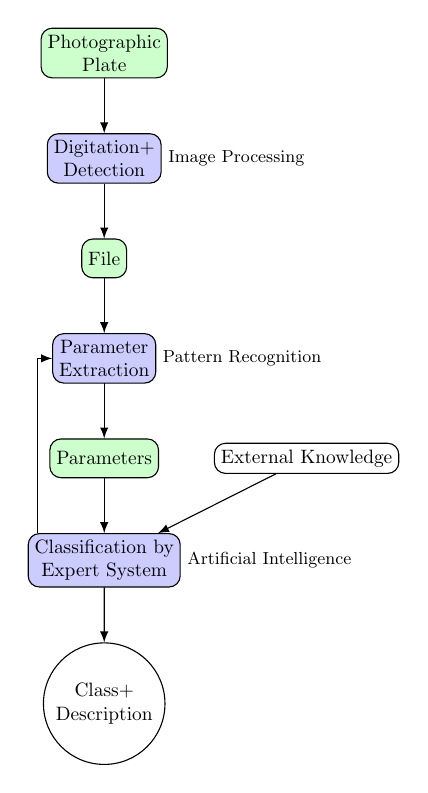
\begin{tikzpicture} [node distance=.7 ,scale=0.7, every node/.style={scale=0.7}]	
		\node[block2] (pplate){Photographic\\Plate};
		\node[block, below = of pplate, label={0: \small{Image Processing}}] (dd) {Digitation+\\Detection};
		\node[block2, below = of dd] (f) {File};
		\node[block, below = of f, label={0: \small{Pattern Recognition}}] (pe) {Parameter\\Extraction};
		\node[block2, below = of pe] (p) {Parameters};
		\node[rectangle, draw, rounded corners, right = of p] (k) {External Knowledge};
		\node[block, below = of p,  label={0: \small{Artificial Intelligence}}] (c) {Classification by\\Expert System};
		\node[circle, align=center, draw, below = of c] (cl) {Class+\\Description};
		\path[line](pplate)--(dd);
		\path[line](dd)--(f);
		\path[line](f)--(pe);
		\path[line](pe)--(p);
		\path[line](p)--(c);
		\path[line](c)--(cl);
		\path[line](c.158)|-(pe.west);
		\path[line](k)--(c);
	\end{tikzpicture}
	\caption{Thonnat's synopsis of automated morphological classification. \parencite[54]{thonnat_toward_1989}}
	\label{fig:syn}
\end{figure}

Barchi et al. cite the importance of morphological classification of galaxies to understand the large-scale structure of the Universe \parencite{barchi_machine_2020}. They categorize decision trees to traditional approach contrasting the more advanced, deep learning technique. One may assume that the deep learning technique would yield more accurate predictions. However, the 94.5\% accuracy is attributed to both the approaches. The focus of my research is training the decision tree and ensemble classifiers. Since the choice of model for advanced techniques yields approximately the same results, I have selected the binary classifier which is more intuitive to understand and the underlying concepts of machine learning are better illuminated.  Barchi et al. only classify elliptical and spiral galaxies.
\parencite{barchi_machine_2020}. In contrast, I add and classify, the `Merger' type galaxies which are the conglomeration of two galaxies colliding into each other.

Another early attempt at automated classification is due to Lahav et al. They compared the classification of 830 galaxies independently classified prior to, by six human classifiers \parencite{lahav_galaxies_1995}. It was concluded that there was unanimous agreement to merely less than 1\% of objects and at best 80\% agreement on T-Type galaxies. It was evident that parameters such as colour, image quality, and size are crucial for the classification and that artificial neural networks could mimic the human experts. This was demonstrated by Ball et al. on the SDSS dataset \parencite*{ball_galaxy_2004} with similar conclusions to Lahav et al \parencite*{lahav_galaxies_1995}. 

\subsection{Ensemble Methods in Astronomical Machine Learning}\label{sec:ema}
Astronomy has been one of the first disciplines to witness the influx of exponential amount of data. A common problem encountered by astronomers as Valentini and Re note is the classification of a vast array of celestial objects according to an established classification scheme \parencite*[579]{way_advances_2012}. For instance, in the case of galaxy classification according to morphology, the Hubble tuning fork is an important starting point. Moreover, another problem in classification is to discover embedded relations among unlabelled or uncategorised objects. Ensemble methods are regarded as a tool rather than off-the-shelf solutions to solve these problems \parencite[579]{way_advances_2012}.

A good example of automated annotation using ensemble methods is the classification of galaxies based on their morphology. Bazell and Aha compared three classifiers namely, Naive Bayes, decision tree, and a neural network that were tasked to predict 800 galaxies \parencite*{bazell_ensembles_2001}. 10-fold cross-validation was performed and average classification errors were collected. The authors observe that the error reduction rate is inversely proportional to the number of target classes, and it varies according to the classifier chosen. Valentini \& Re states the Italian computer scientists state that it is impossible to determine \emph{a priori}, the best classifier component to select for a problem due to the nature of the problem and the nature of the dataset at hand \parencite*[579]{way_advances_2012}. Therefore, they maintain that it is imperative to perform an experimental analysis with different base classifiers to determine their performance. For the morphological classification of galaxies. I have chosen Random Forest as ensemble classifier and assessed its performance against decision tree and with regards to the true classifications.